% Options for packages loaded elsewhere
\PassOptionsToPackage{unicode}{hyperref}
\PassOptionsToPackage{hyphens}{url}
\PassOptionsToPackage{dvipsnames,svgnames,x11names}{xcolor}
%
\documentclass[
  12pt,
]{article}

\usepackage{amsmath,amssymb}
\usepackage{iftex}
\ifPDFTeX
  \usepackage[T1]{fontenc}
  \usepackage[utf8]{inputenc}
  \usepackage{textcomp} % provide euro and other symbols
\else % if luatex or xetex
  \usepackage{unicode-math}
  \defaultfontfeatures{Scale=MatchLowercase}
  \defaultfontfeatures[\rmfamily]{Ligatures=TeX,Scale=1}
\fi
\usepackage{lmodern}
\ifPDFTeX\else  
    % xetex/luatex font selection
    \setmainfont[]{Times New Roman}
\fi
% Use upquote if available, for straight quotes in verbatim environments
\IfFileExists{upquote.sty}{\usepackage{upquote}}{}
\IfFileExists{microtype.sty}{% use microtype if available
  \usepackage[]{microtype}
  \UseMicrotypeSet[protrusion]{basicmath} % disable protrusion for tt fonts
}{}
\makeatletter
\@ifundefined{KOMAClassName}{% if non-KOMA class
  \IfFileExists{parskip.sty}{%
    \usepackage{parskip}
  }{% else
    \setlength{\parindent}{0pt}
    \setlength{\parskip}{6pt plus 2pt minus 1pt}}
}{% if KOMA class
  \KOMAoptions{parskip=half}}
\makeatother
\usepackage{xcolor}
\setlength{\emergencystretch}{3em} % prevent overfull lines
\setcounter{secnumdepth}{5}
% Make \paragraph and \subparagraph free-standing
\makeatletter
\ifx\paragraph\undefined\else
  \let\oldparagraph\paragraph
  \renewcommand{\paragraph}{
    \@ifstar
      \xxxParagraphStar
      \xxxParagraphNoStar
  }
  \newcommand{\xxxParagraphStar}[1]{\oldparagraph*{#1}\mbox{}}
  \newcommand{\xxxParagraphNoStar}[1]{\oldparagraph{#1}\mbox{}}
\fi
\ifx\subparagraph\undefined\else
  \let\oldsubparagraph\subparagraph
  \renewcommand{\subparagraph}{
    \@ifstar
      \xxxSubParagraphStar
      \xxxSubParagraphNoStar
  }
  \newcommand{\xxxSubParagraphStar}[1]{\oldsubparagraph*{#1}\mbox{}}
  \newcommand{\xxxSubParagraphNoStar}[1]{\oldsubparagraph{#1}\mbox{}}
\fi
\makeatother


\providecommand{\tightlist}{%
  \setlength{\itemsep}{0pt}\setlength{\parskip}{0pt}}\usepackage{longtable,booktabs,array}
\usepackage{calc} % for calculating minipage widths
% Correct order of tables after \paragraph or \subparagraph
\usepackage{etoolbox}
\makeatletter
\patchcmd\longtable{\par}{\if@noskipsec\mbox{}\fi\par}{}{}
\makeatother
% Allow footnotes in longtable head/foot
\IfFileExists{footnotehyper.sty}{\usepackage{footnotehyper}}{\usepackage{footnote}}
\makesavenoteenv{longtable}
\usepackage{graphicx}
\makeatletter
\newsavebox\pandoc@box
\newcommand*\pandocbounded[1]{% scales image to fit in text height/width
  \sbox\pandoc@box{#1}%
  \Gscale@div\@tempa{\textheight}{\dimexpr\ht\pandoc@box+\dp\pandoc@box\relax}%
  \Gscale@div\@tempb{\linewidth}{\wd\pandoc@box}%
  \ifdim\@tempb\p@<\@tempa\p@\let\@tempa\@tempb\fi% select the smaller of both
  \ifdim\@tempa\p@<\p@\scalebox{\@tempa}{\usebox\pandoc@box}%
  \else\usebox{\pandoc@box}%
  \fi%
}
% Set default figure placement to htbp
\def\fps@figure{htbp}
\makeatother

\makeatletter
\@ifpackageloaded{caption}{}{\usepackage{caption}}
\AtBeginDocument{%
\ifdefined\contentsname
  \renewcommand*\contentsname{Table of contents}
\else
  \newcommand\contentsname{Table of contents}
\fi
\ifdefined\listfigurename
  \renewcommand*\listfigurename{List of Figures}
\else
  \newcommand\listfigurename{List of Figures}
\fi
\ifdefined\listtablename
  \renewcommand*\listtablename{List of Tables}
\else
  \newcommand\listtablename{List of Tables}
\fi
\ifdefined\figurename
  \renewcommand*\figurename{Figure}
\else
  \newcommand\figurename{Figure}
\fi
\ifdefined\tablename
  \renewcommand*\tablename{Table}
\else
  \newcommand\tablename{Table}
\fi
}
\@ifpackageloaded{float}{}{\usepackage{float}}
\floatstyle{ruled}
\@ifundefined{c@chapter}{\newfloat{codelisting}{h}{lop}}{\newfloat{codelisting}{h}{lop}[chapter]}
\floatname{codelisting}{Listing}
\newcommand*\listoflistings{\listof{codelisting}{List of Listings}}
\makeatother
\makeatletter
\makeatother
\makeatletter
\@ifpackageloaded{caption}{}{\usepackage{caption}}
\@ifpackageloaded{subcaption}{}{\usepackage{subcaption}}
\makeatother

\usepackage{bookmark}

\IfFileExists{xurl.sty}{\usepackage{xurl}}{} % add URL line breaks if available
\urlstyle{same} % disable monospaced font for URLs
\hypersetup{
  pdftitle={Defined System Requirements for the Medication Adherence System},
  colorlinks=true,
  linkcolor={blue},
  filecolor={Maroon},
  citecolor={Blue},
  urlcolor={Blue},
  pdfcreator={LaTeX via pandoc}}


\title{Defined System Requirements for the Medication Adherence System}
\author{Tyler Sapp \and Wyatt Henderson \and Ronaldo
Menendez \and Gustavo Naveto \and Nick Larson}
\date{}

\begin{document}
\maketitle

\renewcommand*\contentsname{Table of contents}
{
\hypersetup{linkcolor=}
\setcounter{tocdepth}{3}
\tableofcontents
}

\section{Defined System Requirements}\label{defined-system-requirements}

\subsection{Functional Requirements}\label{functional-requirements}

\begin{longtable}[]{@{}
  >{\raggedright\arraybackslash}p{(\linewidth - 6\tabcolsep) * \real{0.0533}}
  >{\raggedright\arraybackslash}p{(\linewidth - 6\tabcolsep) * \real{0.1600}}
  >{\raggedright\arraybackslash}p{(\linewidth - 6\tabcolsep) * \real{0.7244}}
  >{\raggedright\arraybackslash}p{(\linewidth - 6\tabcolsep) * \real{0.0622}}@{}}
\toprule\noalign{}
\begin{minipage}[b]{\linewidth}\raggedright
\textbf{Req ID}
\end{minipage} & \begin{minipage}[b]{\linewidth}\raggedright
\textbf{Title}
\end{minipage} & \begin{minipage}[b]{\linewidth}\raggedright
\textbf{Description}
\end{minipage} & \begin{minipage}[b]{\linewidth}\raggedright
\textbf{Priority}
\end{minipage} \\
\midrule\noalign{}
\endhead
\bottomrule\noalign{}
\endlastfoot
\textbf{FR1} & Medication Schedule Retrieval & The system shall retrieve
upcoming medication schedules from the Medication Schedule Store for
each patient. & High \\
\textbf{FR2} & Medication Reminder Dispatch & The system shall
automatically send medication reminders to patients when the scheduled
time is reached. & High \\
\textbf{FR3} & Adherence Confirmation Input & The system shall receive
adherence confirmation from patients, including relevant details such as
timestamp and status. & High \\
\textbf{FR4} & Adherence Record Logging & The system shall record each
adherence confirmation in the Adherence Records Store to track when
medications are taken or missed. & High \\
\textbf{FR5} & Report Generation & The system shall generate adherence
reports by compiling data from the Adherence Records Store (and
optionally the Patient Data Store), store the reports, and send them to
the Healthcare Provider. & Medium \\
\textbf{FR6} & Patient Data Submission & The system shall allow patients
to submit their personal and medical data, which will be validated and
stored in the Patient Data Store. & High \\
\textbf{FR7} & Healthcare Provider Data Access & The system shall allow
healthcare providers to securely retrieve patient data from the Patient
Data Store after verifying their credentials. & High \\
\textbf{FR8} & Reminder Logging & The system shall log all reminder
dispatch events for auditing and troubleshooting purposes. & Medium \\
\end{longtable}

\subsection{Non-Functional
Requirements}\label{non-functional-requirements}

\begin{longtable}[]{@{}
  >{\raggedright\arraybackslash}p{(\linewidth - 6\tabcolsep) * \real{0.0541}}
  >{\raggedright\arraybackslash}p{(\linewidth - 6\tabcolsep) * \real{0.1081}}
  >{\raggedright\arraybackslash}p{(\linewidth - 6\tabcolsep) * \real{0.7748}}
  >{\raggedright\arraybackslash}p{(\linewidth - 6\tabcolsep) * \real{0.0631}}@{}}
\toprule\noalign{}
\begin{minipage}[b]{\linewidth}\raggedright
\textbf{Req ID}
\end{minipage} & \begin{minipage}[b]{\linewidth}\raggedright
\textbf{Title}
\end{minipage} & \begin{minipage}[b]{\linewidth}\raggedright
\textbf{Description}
\end{minipage} & \begin{minipage}[b]{\linewidth}\raggedright
\textbf{Priority}
\end{minipage} \\
\midrule\noalign{}
\endhead
\bottomrule\noalign{}
\endlastfoot
\textbf{NFR1} & Security \& Privacy & All data transactions must be
secured via encryption and proper authentication. The system should
comply with relevant regulations (e.g., HIPAA) where applicable. &
High \\
\textbf{NFR2} & Performance & The system shall deliver medication
reminders and process adherence confirmations within 2 seconds of the
scheduled time. & Medium \\
\textbf{NFR3} & Availability & The system shall maintain an uptime of at
least 99.9\%, ensuring reliable access for patients and healthcare
providers. & High \\
\textbf{NFR4} & Usability & The system shall provide an intuitive,
user-friendly interface that requires minimal training for both patients
and healthcare providers. & Medium \\
\textbf{NFR5} & Scalability & The system shall be designed to scale
efficiently, accommodating an increasing number of patients and
healthcare providers without performance degradation. & Medium \\
\textbf{NFR6} & Maintainability & The system shall be developed using
modular and well-documented code to facilitate ease of maintenance and
future enhancements. & Medium \\
\end{longtable}

\begin{center}\rule{0.5\linewidth}{0.5pt}\end{center}

\subsubsection{How to Use These
Requirements}\label{how-to-use-these-requirements}

\begin{itemize}
\item
  \textbf{Functional Requirements (FRs):}\\
  These describe the specific behaviors and functions of the system. For
  example, FR2 ensures that reminders are sent on time, while FR4 tracks
  adherence events.
\item
  \textbf{Non-Functional Requirements (NFRs):}\\
  These outline the quality attributes of the system. They address
  security, performance, availability, usability, scalability, and
  maintainability, which are critical for a system that handles
  sensitive healthcare data.
\end{itemize}

\subsection{Use Case Diagrams}\label{use-case-diagrams}

Below are two use case diagrams. One for the functional requirements and
one for the non-functional requirements.

\subsubsection{Functional Requirements Use Case
Diagram}\label{functional-requirements-use-case-diagram}

\begin{figure}[H]

{\centering \pandocbounded{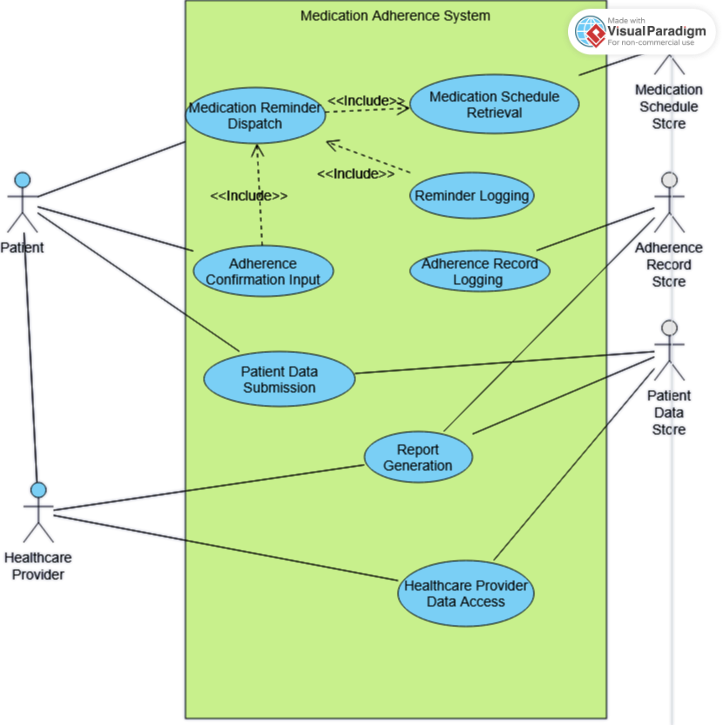
\includegraphics[keepaspectratio]{assets/FR Use Case Diagram.png}}

}

\caption{Use case diagram for functional requirements using Visual
Paradigm}

\end{figure}%

\subsubsection{Non-Functional Use Case
Diagram}\label{non-functional-use-case-diagram}

\begin{figure}[H]

{\centering \pandocbounded{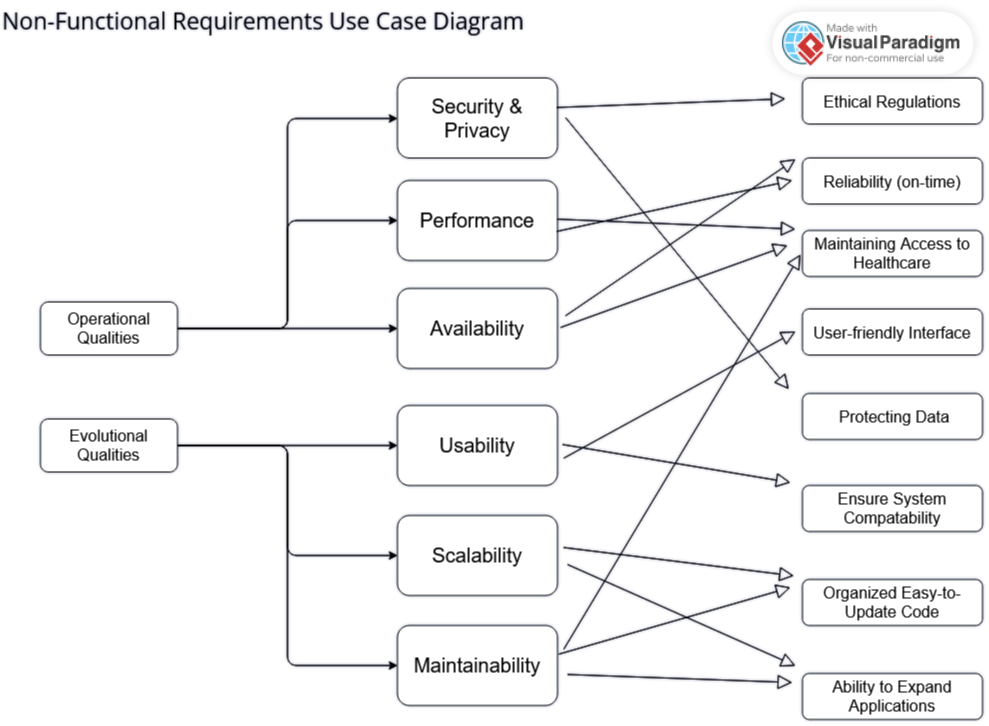
\includegraphics[keepaspectratio]{assets/NFR Use Case Diagram_1.png}}

}

\caption{Use case diagram for non-functional requirements using Visual
Paradigm}

\end{figure}%




\end{document}
